One aspect of Unity that consumes a lot of processing power and time is the instantiation of game objects from prefabs. Because such objects can have a significant runtime memory footprint, creating and destroying them can become a bottleneck as far as performance is concerned. Dickinson's orc example on page 297\cite{optimizationbook} can be applied to many scenarios regarding temporary objects. For Space Shooter, destroyed asteroids instantiate two lesser ones, and those again spawn another two each, for a potential total of additional 6 instantiations per each original asteroid. On top of this, the player weapon spawns new projectiles every time it is fired. The space drones also continuously fire at the player ship, continuously creating a large number of projectile objects. On top of all these, the destruction of an asteroid or drone is accompanied by an explosion effect, which is also a game object containing a particle system.\\
 All these potential gaps in performance could be improved, by creating object pools. Instead of destroying them only to create new ones later, it would be more efficient to simply disable an object that is not needed anymore, and reuse it when needed again. Depending on a case by case basis, one significant question must be answered: How to deal with an insufficient object pool? For example, in a hypothetical explosion object pool of 30 objects, what would happen in case 31 explosions are triggered at once? \\
 One possible answer is to increase the pool by instantiating an additional one. One instantiation, while perhapes less than desirable, is still much better than 31. \\
 Another option can be simply ignoring the 31st explosion, or to generalize, when there are no available objects in the relevant pool, don't do anything. While this can be the best option when targeting performance, it may have a strong undesired impact over the player's experience of the game. \\
 The third option, the middle ground, is instead to reuse the oldest active object in the pool. While it may also have a noticeable, non constant effect on the player, their attention is likely to be focused on the action at hand, therefore an explosion somewhere in the background may go unnoticed, as opposed to destroying an asteroid and sometimes not triggering anything beside the asteroid disappearing and two smaller ones appearing in its place. \\ \\
 It is important when creating an object pool to determine a good estimate of its size, to preserve a balanced memory usage. In the case of Space Shooter, we can determine that since each original asteroid will break into two, and the two pieces will break into another two, the maximum number of asteroids that can be at any one time is four times the original number. However, if the asteroid pool would be initialized with the maximum count, it is very likely that many of the pooled object will remain unused. After experimenting with different values and monitoring the creation of new Asteroids when needed, we have chosen an initial pool 35\% larger than the initial count. With this value we do not have a very high overhead, and extremely rare occurences of additional objects needed. \\
 In regard to the explosion pool, the maximum possible number of instances at any one time would be the maximum possible count of objects that can trigger an explosion. It would be therefore four times the original asteroid count, plus the space drone count. This would be a much too great number of objects to pool, especially for a purely visual component. We will therefore initialize the pool with a static count of 20 explosions for asteroids, and 5 for drones, and reuse the oldest active explosion if there are none available. Because asteroids share their own explosion pool, this will be maintained by the asteroid pool. In the case of hostile drones, the explosion pool will be maintained by the Enemy Manager object. \\
 
 The projectile maximum count can be calculated by dividing the lifetime of the projectile with the fire rate of the weapon, adding one, and multiplying the result with the total count of weapons, calculated separately for each weapon. Because weapon fire should be a reliable game mechanic, we will initialize the projectile pools with the optimal number of projectiles, as reaching the maximum count can be a relatively easy to encounter situation. Every weapon will have its own projectile manager.\begin{figure}
\begin{subfigure}{0.49\textwidth}
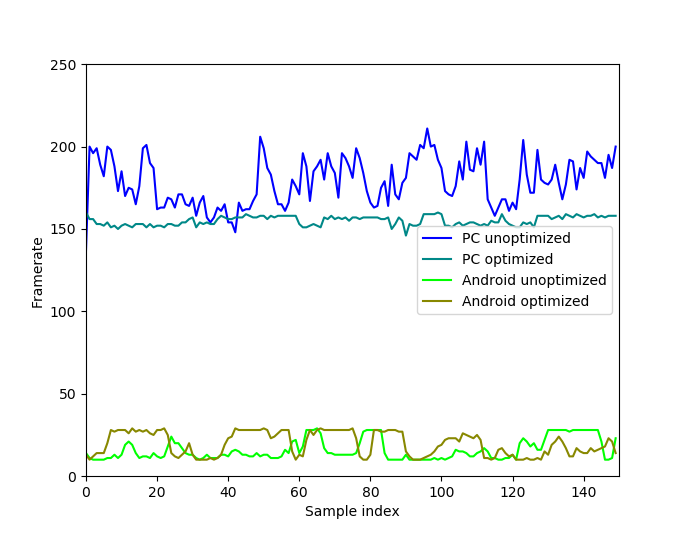
\includegraphics[width = \textwidth, height = 0.66\textwidth]{images/pools}
\end{subfigure}
\caption{Framerate before and after optimization}
\end{figure}
The following changes have been done during the implementation of object pools:
\begin{enumerate}
\item{The asteroid manager does not instantiate Asteroid objects anymore. Instead, objects are requested from the Asteroid pool.}
\item{The Asteroid Pool creates more objects if needed.}
\item{Asteroids have access to the Asteroid Pool in order to instantiate smaller asteroids upon destruction.}
\item{The Object and Enemy Managers both manage their own Explosion Pool objects. Asteroids / Enemies use these pools upon destruction. The Explosion Pool does not create additional objects, instead it disables and recycles the oldest active explosion when needed.}
\item{Each weapon in the game (player weapon and each drone weapon) has its own Projectile Pool. The size of the pool has been calculated based on the weapon's firing rate and the projectile's life span.}
\end{enumerate}
\begin{table}
\caption{Optimization data}
\label{tab:conf}
\begin{minipage}{0.49\textwidth}
\begin{center}
\begin{tabular}{lllll}
Value & PC pre & PC post & Android pre & Android post \\
Mean & 178.94 & 155.04 & 16.01 & 19.70 \\
Std & 14.40 & 2.77 & 6.32 & 7.12 \\
Top 10 mean & 203.00 & 159.20 & 28.10 & 28.60 \\
Bottom 10 mean & 153.80 & 150.30 & 10.00 & 10.00 \\
Min & 137 & 146 & 10 & 10 \\
Max & 211 & 160 & 29 & 29 
\end{tabular}
\bigskip
\end{center} 
\end{minipage}
\end{table}
Looking at the data in figure 7, we notice an overall decrease in the PC performance, shown by a much smoother line however. Implementing the object pooling has come with a decrease of almost 14\%, but with a standard deviation that is only a fifth of the previous value, as can be seen in Table 4.\\
 Meanwhile the Android platform shows yet another slight improvement, with a 23\% increase in the average framerare, with only a slight increase in the standard deviation. While not as even as the PC, this is still a considerable margin, considering the extremely low capabilities of the hardware used. 
